\documentclass[a4paper,14pt]{extarticle}
\usepackage[utf8]{inputenc}
\usepackage[russian]{babel}
\usepackage{graphicx}
\usepackage[top=0.8in, bottom=0.8in, left=0.8in, right=0.8in]{geometry}
\usepackage{pgfplots}
\usepackage{amsmath}
\usepackage{setspace}
\usepackage{titlesec}
\usepackage{float}
\usepackage{chngcntr}
\usepackage{pgfplots}
\usepackage{amsfonts}
\usepackage{pgfplotstable}
\usepackage{multirow}
\usepackage{karnaugh-map}
\usepackage{tikz,xcolor}

\titleformat{\section}[hang]
  {\bfseries}
  {}
  {0em}
  {\hspace{-0.4pt}\large \thesection\hspace{0.6em}}
  
  
\titleformat{\subsection}[hang]
  {\bfseries}
  {}
  {0em}
  {\hspace{-0.4pt}\large \thesubsection\hspace{0.6em}}

%\linespread{1.3} % полуторный интервал
%\renewcommand{\rmdefault}{ftm} % Times New Roman

\newcommand{\nx}{\overline{x}}
\newcommand{\p}{0.31}
\newcommand{\scale}{1.4}

\counterwithin{figure}{section}
\counterwithin{equation}{section}
\counterwithin{table}{section}

\begin{document}
\begin{titlepage}
\centering
Санкт-Петербургский политехнический университет Петра Великого \\
\vspace{0.15cm}
Кафедра компьютерных систем и программных технологий \\
\vspace{6.5cm}

{\centering \textbf{Отчёт по лабораторной работе} \\ 
\vspace{0.15cm}
\textbf{Дисциплина}: Телекоммуникационные технологии \\
\vspace{0.15cm}
\textbf{Тема}: Сигналы телекоммуникационных
систем} \\

\vspace{6.5cm}

\begin{table}[H]
\begin{tabular}{p{\textwidth}@{}r}
{Выполнил студент гр. 33501/4} \hfill {Мальцев  М.С.} \\
{Преподаватель} \hfill {Богач Н.В.} \\
\end{tabular}
\end{table}
\vfill

{\centering Санкт-Петербург \\ 
\vspace{0.15cm}
\today}
\end{titlepage}

\section{Цель работы}

Познакомиться со средствами генерации и визуализации простых сигналов.

\section{Постановка задачи}

В командном окне MATLAB и в среде Simulink промоделировать синусоидальный и прямоугольный сигналы с различными параметрами. Получить их спектры. Вывести на график.

\section{Теоретический раздел}

\section{Ход работы}

\subsection{Моделирование синусоидального сигнала}

При открытие Simulink был выбран шаблон Simple Simulation.

\begin{figure}[H]
\center{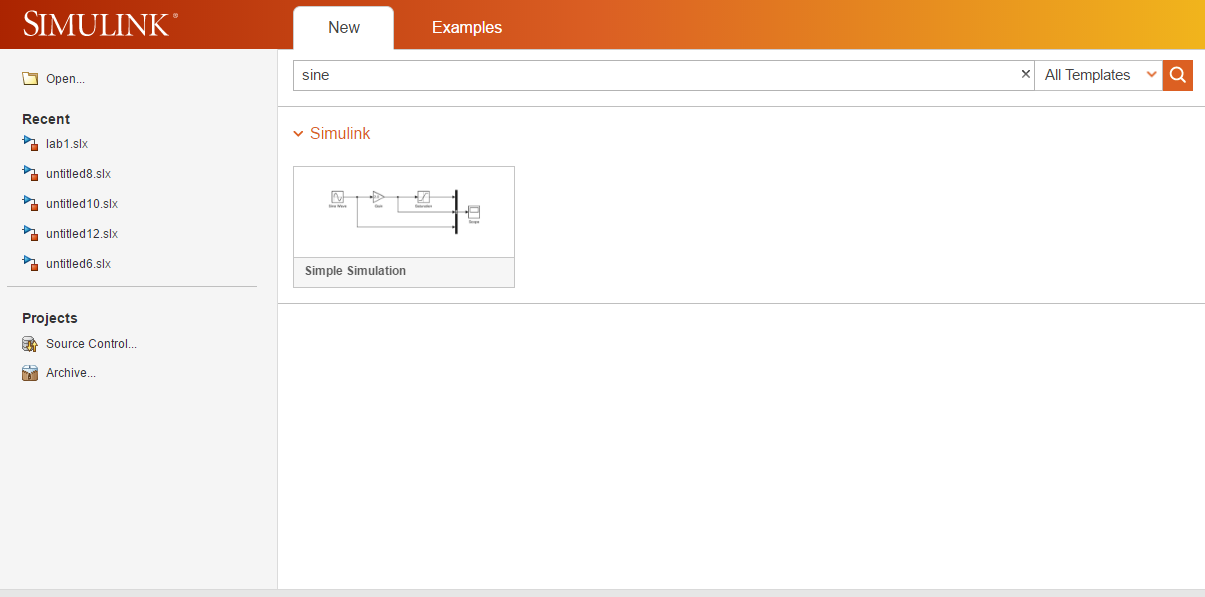
\includegraphics[width=1\linewidth]{img/000.png}}
\caption{Выбор шаблона в начальном окне Simulink.}
\end{figure}

\newpage

В итоге была сгенерирована схема представленная на рисунке \ref{001}.

\begin{figure}[H]
\center{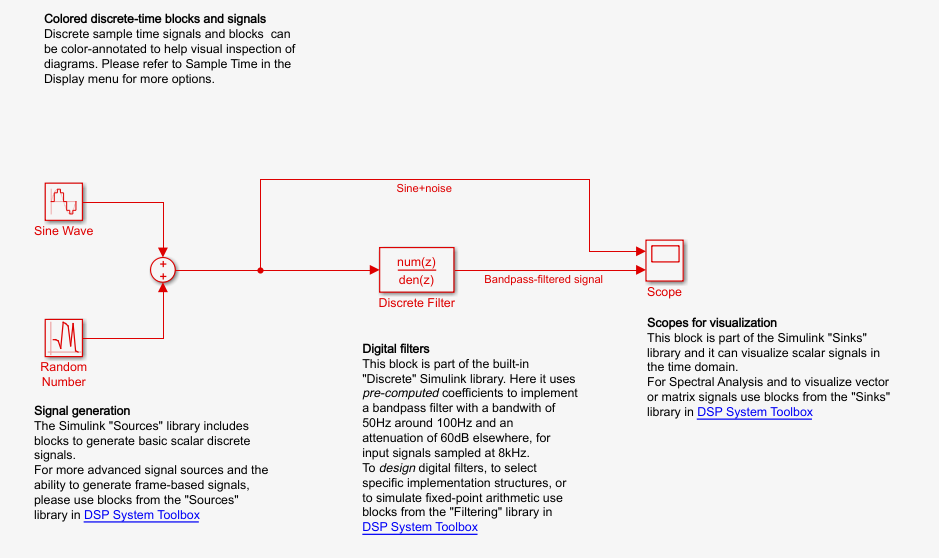
\includegraphics[width=1\linewidth]{img/001.png}}
\caption{Схема автоматически сгенерированная Simulink.}
\label{001}
\end{figure}


Краткое описание назначения элементов:
\begin{itemize}
\item \textbf{Sine Wave} задаёт синусоидальный сигнал с амплитудой 1 и частотой 1 rad/sec
\item \textbf{Gain} усиливает входной сигнал в 2 раза
\item \textbf{Saturation} устанавливает ограничивающие пределы верхний на 0.5 и нижний на -0.5\\
\end{itemize}

Таким образом, при симуляции мы должны увидеть на графике 3 сигнала:
\begin{enumerate}
\item синусоидальный сигнал с амплитудой 1
\item синусоидальный сигнал с амплитудой 2
\item сигнал трапециевидной формы с амплитудой 0.5
\end{enumerate}

Причём, для всех сигналов должен быть одинаковый период,\\ равный 
$\sim$ 6.28 секунды.\\

\newpage

При запуске симуляции получили результаты продемонстрированные на рисунке \ref{002}.

\begin{figure}[H]
\center{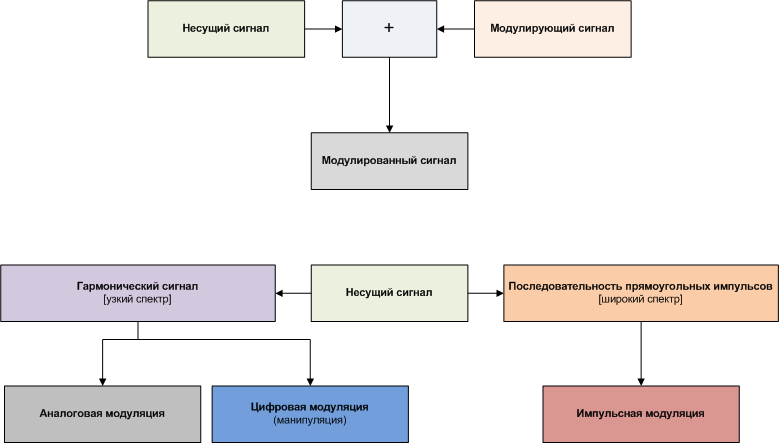
\includegraphics[width=1\linewidth]{img/002.png}}
\caption{Результат симуляция. Окно Scope.}
\label{002}
\end{figure}

Проанализировав результаты симуляции, на соответствие ожиданиям, можно сделать вывод, что она выполнена правильно.

\subsection{Моделирование прямоугольного сигнала}



\section{Выводы}


\end{document}
